\section{静电场}
\gdef\coursepart{静电场、电介质与稳恒电流场}

\begin{frame}{静电场}
电场是存在于电荷周围的、能传递电荷与电荷之间相互作用的物理场。静电场是指各处电场的大小与方向都不变的电场。
静电场的基本性质：散度定理（高斯定理），环路定理（静电场是保守的，可以定义电势）。

几类静电场问题的一般方法：
（1）利用高斯定理/静电场方程的积分解与边界条件求解电场/电势\\
（2）导体问题：唯一性定理和电像法\\
（3）介质问题：利用电介质本构方程和对应边界条件求解\\
（4）静电场的能动角动量：。计算电磁场的场能，利用能动量守恒计算\\
（5）稳恒电流场：KCL/KVL，以及稳恒场方程同解
\src{电磁学讲义\_20251125（张志财）.pdf，第2--5章；基础物理学(3)-电磁学部分教材.pdf，第1--4章。}
\end{frame}

\begin{frame}{电场}
真空中，静止点电荷 $q$ 在距离 $r$ 处产生的电场为
\[
 \vct E=\frac{1}{4\pi\epso}\frac{q}{r^2}\hat{\vct r}.
\]
$\hat{\vct r}$ 从源点指向场点。

电荷连续分布时，可以写为：
\[
 \vct E(\vct r)=\frac{1}{4\pi\epso}\int
 \frac{\vct r-\vct r'}{|\vct r-\vct r'|^3}\,\dd q,
 \quad
 \dd q=\lambda\dd l'\;\hbox{或}\;\sigma\dd S'\;\hbox{或}\;\rho\dd V'.
\]
其中源点为 $\vct r'$，场点为 $\vct r$，
note1：这个公式反映了静电场的一个本质特征：线性可叠加原理。\\
note2：计算时需要关注是否计入了全部的电荷产生的电场\\
note3：计算时常利用对称性时去掉互相抵消的分量，再积分。
\src{DC1(理科).pdf，PDF第19--34页；电磁学讲义\_20251125（张志财）.pdf，PDF第35--43页，第2.1--2.2节。}
\end{frame}

\begin{frame}{高斯定理}
静电场的散度正比于电荷密度：
\[
 \oiint_S\vct E\cdot\dd\vct S=\frac{Q_{\rm in}}{\epso},
 \qquad
 \nabla\cdot\vct E=\frac{\rho}{\epso}.
\]
note1：$\rho$ 和 $Q_{\rm in}$ 都要把自由电荷、感应电荷、极化电荷全部算进去。
note2：用高斯定理求电场一般也需要对称性，一般取高斯面场强在高斯面上大小不变，方向与面垂直。e.g.
\[
 E_{\text{球}}=\frac{Q(r)}{4\pi\epso r^2},\qquad
 E_{\text{柱}}=\frac{\lambda}{2\pi\epso r},\qquad
 E_{\text{面}}=\frac{\sigma}{2\epso}.
\]:
note3：通量为零只说明高斯面内净电荷为零，电荷可能非0。
\src{DC1(理科).pdf，PDF第41--64页；电磁学讲义\_20251125（张志财）.pdf，PDF第44--53页，第2.3--2.4节。}
\end{frame}

\begin{frame}{环路定理}
静电场沿任意闭合曲线的积分为零：
\[
 \oint_C\vct E\cdot\dd\vct l=0,
 \qquad
 \nabla\times\vct E=0.
\]
这说明把电荷沿不同路径从一点移到另一点，电场力做的功相同。\\
由于做功只由两端决定，静电场是保守场，因此可以定义电势。\\
有介质时，环路定理仍然对 $\vct E$ 成立。$\vct D$ 一般不满足环路积分为零，除非介质均匀，或者分界面正好是等势面。
\src{电磁学讲义\_20251125（张志财）.pdf，PDF第54--58页；基础物理学(3)-电磁学部分教材.pdf，第1章。}
\end{frame}

\begin{frame}{电势}
选定参考点的电势为零，
\[
 \varphi(\vct r)=-\int_{\text{参考点}}^{\vct r}\vct E\cdot\dd\vct l,
 \qquad
 \vct E=-\nabla\varphi.
\]
电场指向电势降低的方向。两点之间
\[
 \varphi(B)-\varphi(A)=-\int_A^B\vct E\cdot\dd\vct l.
\]
电荷 $q$ 从 $A$ 移到 $B$，电场力做功 $q[\varphi(A)-\varphi(B)]$。

电荷分布有限、无穷远电势为零时，
\[
 \varphi(\vct r)=\frac{1}{4\pi\epso}\int\frac{\dd q}{|\vct r-\vct r'|}.
\]
没有偶极层时电势连续。$\hat{\vct n}$ 从第 1 侧指向第 2 侧，
\[
 \varphi_1=\varphi_2,\qquad
 \frac{\partial\varphi_1}{\partial n}-\frac{\partial\varphi_2}{\partial n}=\frac{\sigma}{\epso}.
\]
\src{DC1(理科).pdf，PDF第73--103页；电磁学讲义\_20251125（张志财）.pdf，PDF第54--66页，第2.5--2.6节。}
\end{frame}

\begin{frame}{e.g.1.1半球面的电势}
\begin{columns}[T,onlytextwidth]
\begin{column}{0.64\textwidth}
下半球面半径 $R$，面电荷密度 $\sigma$ 均匀。油滴从球心 $O$ 落到碗底 $P$ 刚好停下，只需求两端电势差。极轴向下。球心到面元的距离都是 $R$，半球面积 $2\pi R^2$，
\[
 \varphi_O=\frac{\sigma R}{2\epso}.
\]
$\theta$ 处环带到 $P$ 的距离是 $2R\sin(\theta/2)$，
\[
 \varphi_P=\frac{\sigma R}{2\epso}\int_0^{\pi/2}\cos\frac\theta2\,\dd\theta
 =\frac{\sqrt2\,\sigma R}{2\epso}.
\]
\end{column}
\begin{column}{0.32\textwidth}
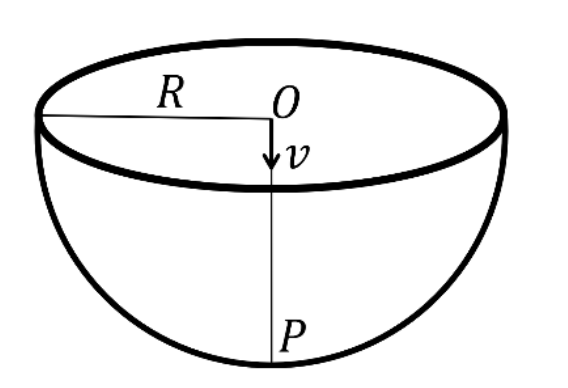
\includegraphics[width=\linewidth]{zhang_hemisphere.png}
\end{column}
\end{columns}
\[
 \varphi_P-\varphi_O=\frac{\sigma R}{2\epso}(\sqrt2-1).
\]
note：环带电量 $2\pi\sigma R^2\sin\theta\,\dd\theta$，弦长 $2R\sin(\theta/2)$。$\sin\theta=2\sin(\theta/2)\cos(\theta/2)$，故被积函数为 $\cos(\theta/2)$。
\src{2025秋基础物理学3期中考试A卷-张志财.pdf，PDF第4页，计算题2；答案PDF第3--4页。}
\end{frame}

\begin{frame}{e.g.1.2油滴的荷质比}
以碗底为重力势能的零点。从 $O$ 到 $P$ 下降的高度是 $R$，油滴在 $P$ 点速度为零：
\[
 \frac12 mv^2+mgR+q\varphi_O=q\varphi_P.
\]
\[
 \boxed{\frac qm
 =\frac{2\epso\left(gR+v^2/2\right)}{\sigma R(\sqrt2-1)}}.
\]
$\sigma>0$ 时碗底电势更高。油滴带正电，下落过程中电势能增加，静电力做负功，初动能和重力势能的减少都转成电势能。

式中有两处 $R$。电势里的 $R$ 是球面半径，用来算弦长和面积；能量式里的 $R$ 是下降高度。重力项 $mgR$ 不能再代进电势公式里约掉。
\src{2025秋基础物理学3期中考试A卷-张志财.pdf，计算题2；答案PDF第3--4页。}
\end{frame}

\begin{frame}{静电场边值关系}
在分界面上取扁柱体，由高斯定理，法向分量的跃变等于面电荷：
\[
 \hat{\vct n}\cdot(\vct E_2-\vct E_1)=\frac{\sigma}{\epso}.
\]
$\hat{\vct n}$ 从第 1 侧指向第 2 侧。其中 $\sigma$ 是界面上的全部面电荷。

再取贴在界面两侧的扁回路，由环路定理，切向分量连续，有：
\[
 \hat{\vct n}\times(\vct E_2-\vct E_1)=0.
\]
note：这一关系在导体和介质中适用，注意导体内部电场=0即可
\src{基础物理学(3)-电磁学部分教材.pdf，第2.7节；电磁学讲义\_20251125（张志财）.pdf，第3、4章的界面关系。}
\end{frame}

\begin{frame}{静电场中的导体}
静电平衡时，导体内电场为零，整块导体是等势体，电荷分布在表面。表面外侧的电场垂直于表面，
\[
 E_t=0,\qquad \epso E_n=\sigma,
\]
$\hat{\vct n}$ 指向导体外部。
note1：可以理解为切向电场如果不为零，电荷还会沿表面移动。\\

note2:空腔的内壁总感应电荷可以用导体内包围空腔的高斯面来求。导体内场为零，所以内壁总电荷等于腔内电荷的负值。\\

note3：孤立导体边界总电荷给定，接地导体边界电势$\varphi=0$给定，分别对应唯一性定理里的两类边界条件。
\src{DC2(理科).pdf，PDF第1--25页；电磁学讲义\_20251125（张志财）.pdf，PDF第67--76页，第3.1--3.2节。}
\end{frame}

\begin{frame}{唯一性定理}
导体上的电荷分布与电场互相决定，会导致思考与计算非常困难。一般的做法是把导体内部从求解区域里除掉，只求解剩下的空间，然后把导体当做边界条件。\\
由静电场唯一性定理：区域内电荷分布已经给定时，再给出下列边界条件之一，电势就唯一确定。电势可以差一个常数，电场则完全确定。
\begin{enumerate}
\item 给定边界上各处的电势。
\item 边界是等势面，并且给定面电荷密度，或给定每块导体的总电荷。
\item 前两种混合。
\end{enumerate}
因此，只要构造出的电势满足泊松方程和这些边界条件，它就是静电场的解。

e.g.静电屏蔽中，空腔的边界条件只由腔内电荷和内壁总电荷决定，腔外电荷改变不了它，也就改变不了腔内的场。导体接地时，外表面的边界条件是电势为零，腔内电荷的多少也不影响腔外的场。
\src{电磁学讲义\_20251125（张志财）.pdf，PDF第77--80页，第3.3节，定理3.1。}
\end{frame}

\begin{frame}{电像法}
在待求区域的外面放一个或几个假想电荷，称为镜像电荷。只要满足以下条件：
\begin{enumerate}
\item 镜像电荷不进入待求区域，区域内原有的电荷分布不变。
\item 真实电荷与镜像电荷合在一起，使导体表面成为等势面，而且电势等于题目给定的值。
\end{enumerate}
这样得到的电势满足区域内的泊松方程和边界条件。由唯一性定理就是这个区域的解。
note1：求解电像法时必须注意区分“物理空间”和“镜像空间”，一个物理空间上的镜像电荷必须存在于与物理空间正交的镜像空间里，但其产生的电场只在物理空间中有意义\\
note2：求表面电荷仍用$\sigma=\epso E_n$，电场取这个区域里的解。求真实电荷受到的力，只用镜像电荷在它位置上产生的场。\\
note3:电像法本质是凑解要先知道哪种电荷分布能给出所需形状的等势面，所以只适合平面、球面等少数边界。
\src{电磁学讲义\_20251125（张志财）.pdf，PDF第80--82页，第3.4节；基础物理学(3)-电磁学部分教材.pdf，第2.8节。}
\end{frame}

\begin{frame}{接地导体平面}
点电荷 $q$ 在无限大接地导体平面上方，距离为 $d$，平面电势为零。待求区域是平面上方。

在平面下方对称位置放镜像电荷 $-q$。等量异号的两个点电荷，中垂面电势为零，正好与接地平面重合，镜像电荷又在区域外面。上半空间的电势就是
\[
 \varphi=\frac{1}{4\pi\epso}\left(
 \frac{q}{R_+}-\frac{q}{R_-}\right),
\]
$R_+$、$R_-$ 分别是到 $q$ 和到 $-q$ 的距离。

平面上的感应电荷由外侧法向电场给出，
\[
 \sigma=-\frac{qd}{2\pi(r^2+d^2)^{3/2}}.
\]
对整个平面积分，总感应电荷等于 $-q$。正电荷把负电荷吸到近侧，密度在垂足处最大。
\src{电磁学讲义\_20251125（张志财）.pdf，PDF第81--82页，例3.5；基础物理学(3)-电磁学部分教材.pdf，例2.12。}
\end{frame}

\begin{frame}{镜像电荷的受力}
$q$ 受到的力等于镜像电荷 $-q$ 对它的库仑力。两者相距 $2d$，
\[
 F_d=-\frac{q^2}{16\pi\epso d^2}.
\]
$d$ 增大的方向离开平面，负号表示吸向平面。计算力时用镜像电荷的场，不再乘 $1/2$。

能量不能把 $q$ 和 $-q$ 当成两个真实点电荷。两个真实点电荷的相互作用能是 $-q^2/(8\pi\epso d)$，那是把两个电荷都从无穷远搬来的功。现在 $-q$ 是假想的，平面上的感应电荷随着 $q$ 一起产生。

对真实电荷只取一半：
\[
 W=\frac12 q\varphi_{\text{镜像}}
 =-\frac{q^2}{16\pi\epso d}.
\]
$\varphi_{\text{镜像}}$ 是 $-q$ 在 $q$ 处产生的电势。把 $q$ 从无穷远缓慢移到 $d$，外力与电场力平衡，外力做的功也是这个值。\alert{能量有 $1/2$，力没有 $1/2$。}
\src{电磁学讲义\_20251125（张志财）.pdf，例3.5；2025秋基础物理学3期中考试A卷-张志财.pdf，填空6，答案为 $-q^2/(16\pi\epso d)$。}
\end{frame}

\begin{frame}{导体球}
点电荷 $q$ 到球心的距离为 $a$，导体球半径为 $R$。两个异号、电量不相等的点电荷，零电势面是一个球面，球面把它们隔开。由此确定镜像电荷。

接地时，在球心与 $q$ 的连线上、离球心 $b=R^2/a$ 处放
\[
 q'=-\frac{R}{a}q.
\]
待求的那一侧只用 $q$ 和 $q'$。球外问题中 $q'$ 在球内；空腔问题中电荷在球内，$q'$ 就放到球外。球面上总感应电荷等于 $q'$。

球不接地、原来又不带电时，球面仍是等势面，但电势不一定为零，总电荷必须为零。再在球心放 $q''=(R/a)q$。它在球面上的电势是常数，不破坏等势，又与 $q'$ 抵消。这就是唯一性定理要求的“给定总电荷”。

$q$ 受到的力只来自镜像电荷。接地球把它吸向球心。孤立的中性球上，球心处的同号镜像向外推，球内的异号镜像向里拉，总效果仍是吸引。
\src{电磁学讲义\_20251125（张志财）.pdf，PDF第83--86页，例3.7。}
\end{frame}

\begin{frame}{电介质}
电介质在电场中会被极化。无极分子的正负电荷中心被拉开，有极分子的电矩转向电场方向，内部产生偶极子分布。宏观上用极化强度 $\vct P$ 表示，它等于单位体积内分子电偶极矩的矢量和，单位与面电荷密度相同。

极化电荷由 $\vct P$ 决定。$\hat{\vct n}$ 从介质指向外部，
\[
 \rho_b=-\nabla\cdot\vct P,\qquad
 \sigma_b=\vct P\cdot\hat{\vct n}.
\]
$\vct P$ 均匀时，内部正负电荷首尾相接，体电荷为零，电荷只出现在表面。$\vct P$ 沿外法向穿出的地方出现正的束缚面电荷。

各向同性线性介质中，极化与介质内的总电场成正比：
\[
 \vct P=\epso\chi_e\vct E,\qquad \chi_e>0.
\]
$\chi_e$ 是电极化率。注意这里的 $\vct E$ 是介质里的总场，包含极化电荷自己产生的场。
\src{电磁学讲义\_20251125（张志财）.pdf，PDF第89--95页，第4.1--4.2节；DC2(理科).pdf，PDF第47--65页。}
\end{frame}

\begin{frame}{电位移}
总电场的高斯定理右端包含全部电荷。极化电荷又由 $\vct P$ 决定，$\vct P$ 又依赖总电场，直接用 $\vct E$ 往往解不下去。于是我们引入电位移矢量：
\[
 \vct D=\epso\vct E+\vct P,
\]
这样在高斯定理积分中，把极化电荷移到左边：
\[
 \oiint_S\vct D\cdot\dd\vct S=Q_{f,\rm in},
 \qquad
 \nabla\cdot\vct D=\rho_f.
\]
$\vct D$ 的通量只和自由电荷有关，而一个介质体系的自由电荷是容易确定的。

在线性各向同性介质中 $\vct D=\varepsilon\vct E$，
\[
 \varepsilon=\varepsilon_r\epso=\epso(1+\chi_e),\qquad
 \vct P=\left(1-\frac{\epso}{\varepsilon}\right)\vct D.
\]
$\varepsilon$ 是介电常量，$\varepsilon_r$ 是相对介电常量。

环路定理只对$\vct E$成立。$\vct D$ 的环流一般不为零。只有介质分区均匀，并且分界面与等势面重合时，$\vct D$ 才和真空中的 $\epso\vct E$ 满足同一组方程。
\src{电磁学讲义\_20251125（张志财）.pdf，PDF第98--102页，第4.3节。}
\end{frame}

\begin{frame}{电介质的边值关系}
$\hat{\vct n}$ 从介质 1 指向介质 2。界面上的自由面电荷为 $\sigma_f$ 时，
\[
 \hat{\vct n}\times(\vct E_2-\vct E_1)=0,
 \qquad
 \hat{\vct n}\cdot(\vct D_2-\vct D_1)=\sigma_f.
\]
电势仍然连续。线性介质中，第二条就是 $\varepsilon_2 E_{2n}-\varepsilon_1 E_{1n}=\sigma_f$。

没有自由面电荷时 $D_n$ 连续，$E_n$ 一般不连续。切向电场连续，$D_t=\varepsilon E_t$不一定连续。

净束缚面电荷为：
\[
 \sigma_b=(\vct P_1-\vct P_2)\cdot\hat{\vct n}.
\]
\src{基础物理学(3)-电磁学部分教材.pdf，PDF第76--77页，第2.7节；2025秋 A 卷选择4。}
\end{frame}

\begin{frame}{均匀极化球}
\begin{columns}[T,onlytextwidth]
\begin{column}{0.70\textwidth}
半径为 $R$ 的球，内部 $\vct P$ 是常矢量，球外为真空。体束缚电荷为零，表面
\[
 \sigma_b=P\cos\theta.
\]
余弦分布的面电荷在球内产生均匀场。由球面电势连续和 $E_r$ 的跃变，我们有，
\[
 \vct E_{\rm in}=-\frac{\vct P}{3\epso}.
\]
这个场与$\vct P$相反，称为退极化场。
\end{column}
\begin{column}{0.26\textwidth}
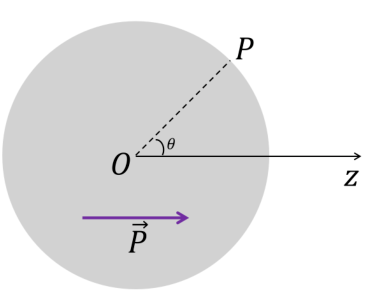
\includegraphics[width=\linewidth]{m1_uniform_polarization.png}
\end{column}
\end{columns}
总电偶极矩 $\vct p=(4\pi R^3/3)\vct P$。球外电场等效于这个球心处偶极子产生的场。
\[
 \vct E_{\rm out}
 =\frac{3(\vct p\cdot\hat{\vct r})\hat{\vct r}-\vct p}{4\pi\epso r^3}.
\]
\src{电磁学讲义\_20251125（张志财）.pdf，PDF第96页，例4.1；基础物理学(3)-电磁学部分教材.pdf，例2.5。}
\end{frame}

\begin{frame}{径向极化球}
\begin{columns}[T,onlytextwidth]
\begin{column}{0.72\textwidth}
球内$\vct P=f(r)\hat{\vct r}$，没有自由电荷，球外是真空。束缚电荷为
\[
 \rho_b=-\frac{1}{r^2}\frac{\dd}{\dd r}[r^2 f(r)],
 \qquad
 \sigma_b=f(R).
\]
取同心球面。自由电荷为零，对称性给出$D_r=0$，于是
\[
 \vct E_{\rm in}=-\frac{f(r)}{\epso}\hat{\vct r},
 \qquad
 \vct E_{\rm out}=0.
\]
note：这个结果只用了 $\vct D=\epso\vct E+\vct P$ 和自由电荷的高斯定理，不需要介质是线性的。
\end{column}
\begin{column}{0.24\textwidth}
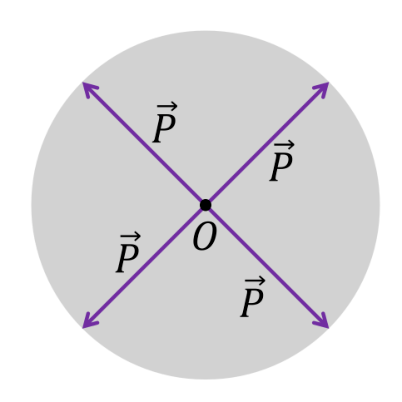
\includegraphics[width=\linewidth]{m1_radial_polarization.png}
\end{column}
\end{columns}
若 $f(r)=P$ 为常数，则 $\rho_b=-2P/r$，体电荷并不为零。球内的体电荷与球面电荷总量抵消，所以球外场为零。
\src{电磁学讲义\_20251125（张志财）.pdf，PDF第96--97页，例4.2；2025秋 A 卷填空2，答案 $\vct E=-f(r)\hat{\vct r}/\epso$。}
\end{frame}

\begin{frame}{匀强外场中的介质球}
均匀外场 $\vct E_0$ 中放入半径 $R$、介电常量 $\varepsilon$ 的线性介质球，球外为真空。均匀外场使球的极化也是均匀的，可以直接用上一节的退极化场：
\[
 \vct E_{\rm in}=\vct E_0-\frac{\vct P}{3\epso},
 \qquad
 \vct P=(\varepsilon-\epso)\vct E_{\rm in}.
\]
第二式里的电场是球内总场。联立后
\[
 \boxed{\vct E_{\rm in}=\frac{3\epso}{\varepsilon+2\epso}\vct E_0},
 \qquad
 \vct P=\frac{3\epso(\varepsilon-\epso)}{\varepsilon+2\epso}\vct E_0.
\]
球外是原来的均匀场加上球心偶极子的场，
\[
 \vct p=4\pi\epso R^3\frac{\varepsilon-\epso}{\varepsilon+2\epso}\vct E_0.
\]
这个势在球面上连续，法向 $\vct D$ 也连续，所以它就是唯一解。

$\varepsilon=\epso$ 时没有极化。$\varepsilon\to\infty$ 时球内场趋于零，$\vct p\to 4\pi\epso R^3\vct E_0$，回到不带电的导体球。导体球可以看成电像法中放在球心的偶极子。
\src{基础物理学(3)-电磁学部分教材.pdf，例2.8；电磁学讲义\_20251125（张志财）.pdf，习题3.3、例4.1。}
\end{frame}

\begin{frame}{双层球壳}
同心球形电容器，内导体半径 $a$，外导体内半径 $b$，介质在 $r=c$ 处分成两层，$a<c<b$，介电常量分别为 $\varepsilon_1$、$\varepsilon_2$。内导体自由电荷为 $Q$。

分界面是球面，与径向电场垂直，也与等势面重合。取同心球面，通量只由自由电荷决定，两层中
\[
 D_r=\frac{Q}{4\pi r^2},\qquad
 E_i=\frac{D_r}{\varepsilon_i}.
\]
介电常量大的一层场强小。两层电压相加，相当于串联：
\[
 C=4\pi\Big/
 \left[\frac1{\varepsilon_1}\left(\frac1a-\frac1c\right)
 +\frac1{\varepsilon_2}\left(\frac1c-\frac1b\right)\right].
\]
均匀介质内部 $\nabla\cdot\vct P=0$，束缚电荷只在表面上。$\vct P=(1-\epso/\varepsilon)\vct D$，
\[
 \sigma_b(a)=-P_1(a),\;
 \sigma_b(c)=P_1(c)-P_2(c),\;
 \sigma_b(b)=P_2(b).
\]
note：内表面的外法向指向球心，所以带负号。
\src{基础物理学(3)-电磁学部分教材.pdf，第2.7.5节，界面与等势面重合；张讲义习题4.3为同轴情形。}
\end{frame}

\begin{frame}{两个半球}
球形电容器内外半径 $a$、$b$，两导体带电 $\pm Q$。过球心的平面把介质分成两个半球，介电常量分别为 $\varepsilon_1$、$\varepsilon_2$。

分界面与径向电场平行。切向电场连续，两半球中的 $E$ 相同，都沿径向。一个闭合球面上，两侧电位移的通量相加等于 $Q$：
\[
 E=\frac{Q}{2\pi(\varepsilon_1+\varepsilon_2)r^2},\qquad
 D_i=\varepsilon_i E.
\]
两半球的 $D$ 不同，自由电荷在 $D$ 较大的一侧更多。电势差由同一个 $E$ 从 $a$ 积到 $b$，电容相当于并联：
\[
 C=\frac{2\pi(\varepsilon_1+\varepsilon_2)}{1/a-1/b}.
\]
$\varepsilon_1=\varepsilon_2=\varepsilon$ 时回到 $4\pi\varepsilon/(1/a-1/b)$。平界面上 $\vct P$ 与法向垂直，$\sigma_b=0$。
note：一般来说等势面平行界面方向时，D相等；等势面垂直界面方向时，E相等，但是本质还是电磁场的边界条件。
\src{基础物理学(3)-电磁学部分教材.pdf，例2.9，界面与电场线重合。}
\end{frame}

\begin{frame}{介质无穷大平面}
上半空间介电常量为 $\varepsilon_1$，下半空间为 $\varepsilon_2$。点电荷 $q$ 在界面上方距离 $d$ 处，界面没有自由电荷。

上半空间用 $q$ 和下侧对称位置的镜像 $q'$。下半空间用放在 $q$ 原位置的 $q''$。两组镜像不能放进同一个区域。
\[
 \varphi_1=\frac{1}{4\pi\varepsilon_1}
 \left(\frac{q}{R_+}+\frac{q'}{R_-}\right),
 \qquad
 \varphi_2=\frac{1}{4\pi\varepsilon_2}\frac{q''}{R_+}.
\]
电势连续、$D_z$ 连续，解出
\[
 q'=\frac{\varepsilon_1-\varepsilon_2}{\varepsilon_1+\varepsilon_2}q,\qquad
 q''=\frac{2\varepsilon_2}{\varepsilon_1+\varepsilon_2}q.
\]
$q$ 的受力只用 $q'$。$\varepsilon_2>\varepsilon_1$ 时电荷被吸向介质。$\varepsilon_2\to\infty$ 且 $\varepsilon_1=\epso$ 时回到接地导体平面。
\src{电磁学讲义\_20251125（张志财）.pdf，习题4.6；基础物理学(3)-电磁学部分教材.pdf，例2.13。}
\end{frame}

\begin{frame}{界面上的点电荷}
\begin{columns}[T,onlytextwidth]
\begin{column}{0.73\textwidth}
$z>0$ 为真空，$z<0$ 的相对介电常量为 $\varepsilon_r$。$q_1$ 在 $z=d$，$q_2$ 在 $z=-d$，界面没有自由面电荷。两个电荷分别做电像，再在各自区域里叠加。
\[
 q_1'=\frac{1-\varepsilon_r}{1+\varepsilon_r}q_1,\quad
 q_1''=\frac{2\varepsilon_r}{1+\varepsilon_r}q_1.
\]
对 $q_2$ 把两侧介电常量对调：
\[
 q_2'=\frac{\varepsilon_r-1}{\varepsilon_r+1}q_2,\quad
 q_2''=\frac{2}{1+\varepsilon_r}q_2.
\]
\end{column}
\begin{column}{0.24\textwidth}
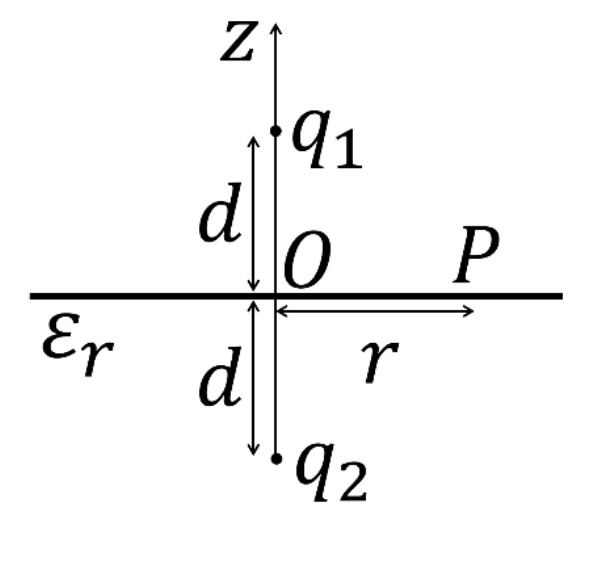
\includegraphics[width=\linewidth]{zhang_dielectric.png}
\end{column}
\end{columns}
上半空间用 $q_1$ 和位于 $z=-d$ 的 $q_1'+q_2''$。受力去掉 $q_1$ 自己的场，这两个电荷与它相距 $2d$，向上为正：
\[
 \boxed{F_{1z}
 =\frac{(1-\varepsilon_r)q_1^2+2q_1 q_2}
 {16\pi\epso(1+\varepsilon_r)d^2}}.
\]
$\varepsilon_r=1$ 时回到库仑力。$\varepsilon_r\to\infty$ 时 $q_1$ 的镜像趋于 $-q_1$，与接地平面一致。
\src{2025秋 A 卷计算题3；答案 PDF 第4--6页。单电荷模型为张讲义习题4.6。}
\end{frame}

\begin{frame}{界面上的束缚电荷}
束缚面电荷用介质一侧的电场。真空与介质的界面上，介质的外法向是 $+\hat{\vct z}$，
\[
 \sigma_b=P_z=\epso(\varepsilon_r-1)E_z(0^-).
\]
下半空间的电势用 $q_2$ 和位于 $z=d$ 的 $q_2'+q_1''$，分母里的介电常量是 $\varepsilon_r\epso$。在 $z=0$ 处，
\[
 E_z(0^-)=\frac{d\,(q_2-\varepsilon_r q_1)}
 {2\pi\epso\varepsilon_r(1+\varepsilon_r)L^3},
\]
$L=\sqrt{r^2+d^2}$。因此
\[
 \boxed{\sigma_b(r)
 =\frac{(q_1-q_2/\varepsilon_r)\,d\,(1-\varepsilon_r)}
 {2\pi(1+\varepsilon_r)(r^2+d^2)^{3/2}}}.
\]
$\varepsilon_r=1$ 时 $\sigma_b=0$。$q_2=0$ 时回到单个点电荷对着介质半空间的结果。

$q_1''$、$q_2''$ 只代表另一侧对这一侧的影响，不能把两侧的镜像电荷放进同一个库仑积分。
\src{2025秋 A 卷计算题3；答案 PDF 第4页，$\sigma'$ 与上式相同。}
\end{frame}

\begin{frame}{电势能}
外场已经给定、不因这个电荷而改变时，电荷在外场中的电势能是
\[
 W=q\varphi_{\text{外}}.
\]
电场力做的功等于电势能的减少。这里没有 $1/2$，$\varphi_{\text{外}}$ 也不包括该电荷自己的电势。产生外场的那些电荷，它们自己的能量不算在内。

电偶极矩 $\vct p$ 从负电荷指向正电荷。永久偶极子的大小和方向都固定时，它在外场中的电势能和力矩是
\[
 W=-\vct p\cdot\vct E_{\text{外}},
 \qquad
 \vct\tau=\vct p\times\vct E_{\text{外}}.
\]
匀强外场中合力为零，力矩使 $\vct p$ 转向电场方向。$W$ 仍然没有 $1/2$，因为外场是维持住的，不是和偶极子一起建立的。
\src{电磁学讲义\_20251125（张志财）.pdf，PDF第54--66页、第105页，第2.6节、第5.1节开头。}
\end{frame}

\begin{frame}{静电能}
电荷体系的静电能，等于把各电荷从无穷远处逐个搬到指定位置时，外力克服电场力做的功。

两个点电荷：先放好 $q_1$，不做功；再搬来 $q_2$，做功 $q_2\varphi_1$。
\[
 W=\frac{q_1 q_2}{4\pi\epso r}
 =\frac12(q_1\varphi_1+q_2\varphi_2).
\]
$\varphi_1$ 是另一个电荷在 $q_1$ 处的电势。$n$ 个点电荷写成 $W=\frac12\sum_i q_i\varphi_i$ 时，每一对相互作用出现两次，所以有 $1/2$。

连续分布时，电荷是逐渐加上去的，后加上的电荷面对已经升高的电势，
\[
 W=\frac12\int\rho\varphi\,\dd V
 =\frac{\epso}{2}\int E^2\,\dd V.
\]
有限大小的电荷分布上两个式子相等，并包含自能。点电荷自能发散，相互作用只保留电荷之间的项。
\src{电磁学讲义\_20251125（张志财）.pdf，PDF第105--109页，第5.1--5.2节，式(5.8)(5.9)(5.19)。}
\end{frame}

\begin{frame}{有介质时的能量}
搬动的是自由电荷，极化随之一起建立。电动力学里，元功是
\[
 \delta W=\int\vct E\cdot\delta\vct D\,\dd V.
\]
线性介质 $\vct D=\varepsilon\vct E$，积分后
\[
 W=\frac12\int\vct D\cdot\vct E\,\dd V
 =\frac12\int\rho_f\varphi\,\dd V.
\]
$\varphi$ 含自由电荷和极化电荷。铁电体不能用这个 $1/2$。$Q^2/(2C)$ 和 $CU^2/2$ 都是这个 $W$。

用 $\vct D=\epso\vct E+\vct P$ 拆开，
\[
 W=\int\frac{\epso E^2}{2}\,\dd V
 +\int\frac{\vct P\cdot\vct E}{2}\,\dd V.
\]
前一项等于对全部电荷作 $\frac12\int\rho\varphi\,\dd V$。后一项来自建立极化。中文教材对这两项的叫法并不一致，就不要纠结语言细节了。
\src{电磁学讲义\_20251125（张志财）.pdf，第5.3节，式(5.36)(5.39)(5.40)。电动力学中元功为 $\vct E\cdot\delta\vct D$。}
\end{frame}

\begin{frame}{偶极子的能量}
$\displaystyle\int\frac{\vct P\cdot\vct E}{2}\,\dd V$ 是上一页 $W$ 的第二项。永久偶极子的势能另写。

$\vct p$ 固定、外场由外界维持时，
\[
 W=-\vct p\cdot\vct E_{\text{外}}.
\]
这里没有 $1/2$。

诱导偶极子 $\vct p=\alpha\vct E$ 是场逐渐拉出来的。拉开电荷贡献 $\vct p\cdot\vct E/2$，与外场相互作用是 $-\vct p\cdot\vct E$，合起来
\[
 W=-\frac12\vct p\cdot\vct E=-\frac12\alpha E^2.
\]
电容器里储存多少能，用 $\frac12\int\vct D\cdot\vct E\,\dd V$。偶极子趋向强场还是弱场，用这里的 $W$：永久偶极子是 $-\vct p\cdot\vct E$，诱导偶极子是 $-\alpha E^2/2$。两处都是强场更低。
\src{电磁学讲义\_20251125（张志财）.pdf，式(5.42)--(5.45)。}
\end{frame}

\begin{frame}{电容}
两个导体分别带电 $+Q$、$-Q$，电势差为 $U=\varphi_+-\varphi_-$。电容定义为
\[
 C=\frac QU.
\]
电容只由几何形状和介质决定，表示同样的电势差下能储存电荷的能力；在同样的电势下，储存的能量 $CU^2/2$ 也更多。电荷固定时，能量是 $Q^2/(2C)$，$C$ 大则能量小。

求解电容的方法是假设法，先假设带有一定的电荷或具有一定的电势，求 $\vct D$ 或 $\vct E$，再沿电场积分得到 $U$。一些常见的结果有：
\[
 C_{\text{平板}}=\frac{\varepsilon S}{d},\qquad
 C_{\text{球}}=4\pi\varepsilon\frac{ab}{b-a},\qquad
 C_{\text{同轴}}=\frac{2\pi\varepsilon l}{\ln(b/a)}.
\]
电容的串并联行为可以将1/c与R类比
\src{电磁学讲义\_20251125（张志财）.pdf，PDF第114--118页，第5.4节。2025秋 A 卷选择6的答案是 A、C。}
\end{frame}

\begin{frame}{能量法求力}
设 $x$ 是介质插入的深度，$x$ 增大表示介质更进入电容器。$F_x$ 是电场对介质的力。

断开电源时 $Q$ 不变，没有能量从电源进来。电场力做正功，静电能减少：
\[
 F_x=-\left(\frac{\partial W}{\partial x}\right)_Q
 =\frac{Q^2}{2C^2}\frac{\dd C}{\dd x}.
\]
接在恒压电源上时 $U$ 不变。电源做功 $U\dd Q$，其中一部分成为静电能，其余是电场对介质做的功：
\[
 U\dd Q=\dd W+F_x\dd x.
\]
由 $\dd Q=U\dd C$、$\dd W=\frac12 U^2\dd C$，
\[
 F_x=\frac12 U^2\frac{\dd C}{\dd x}
 =+\left(\frac{\partial W}{\partial x}\right)_U.
\]
两个式子的符号不同，是因为 $Q$ 不变时能量随 $C$ 增大而减小，$U$ 不变时能量随 $C$ 增大而增大。$\dd C/\dd x>0$ 时都有 $F_x>0$，介质都被吸进去。拉出介质时，外力与 $F_x$ 反向。
\src{DC3(理科).pdf，PDF第1--34页；2025秋 A 卷选择9，恒压插入时介质受吸引力。}
\end{frame}

\begin{frame}{e.g.2.1能量法求抽出电容器介质板}
平行板长 $l$、宽 $b$、间距 $d$。介质厚度等于 $d$，介电常量为 $\varepsilon$，已经插入深度 $x$。忽略边缘对电容数值的影响，
\[
 C=\frac{\varepsilon bx}{d}+\frac{\epso b(l-x)}{d},
 \qquad
 \frac{\dd C}{\dd x}=\frac{(\varepsilon-\epso)b}{d}.
\]
两块极板是等势体，介质区和空气区的电势差相同，相当于并联。
\[
 F_x=
\begin{cases}
\dfrac{Q^2}{2C^2}\dfrac{(\varepsilon-\epso)b}{d}, & Q\ \text{不变},\\[10pt]
\dfrac{U^2}{2}\dfrac{(\varepsilon-\epso)b}{d}, & U\ \text{不变}.
\end{cases}
\]
$U$ 不变时 $E=U/d$ 不随 $x$ 改变，$F_x$ 是常数。$Q$ 不变时 $C$ 随插入增大，$E=Q/(Cd)$ 变小，吸力也变小。

$Q$ 不变，把板拉出：$C$ 减小，$W=Q^2/(2C)$ 增大，增加的能量等于外力做的功。

$U$ 不变，把板拉出：$W=CU^2/2$ 减小，外力仍然做正功。电荷流回电源，电源增加的能量等于外力的功加上电容器减少的静电能。
\src{由虚功原理与平行板电容公式计算。恒压时介质被吸入，与 2025 秋 A 卷选择9一致。}
\end{frame}

\begin{frame}{e.g.2.2电压强法求抽出电容器介质板}
介质从侧面插入时，端面与极板垂直，板间电场与这个端面平行。端面上 $\vct P$ 的法向分量为零，$\sigma_b=0$，不能写成 $\sigma_b E$。吸力来自边缘处的电场对极化电荷的作用，合起来相当于一个压强
\[
 p=\frac12(\varepsilon-\epso)E^2.
\]
方向指向空气一侧，也就是把介质拉进电容器。端面面积为 $bd$，
\[
 F_x=p\,bd=\frac12(\varepsilon-\epso)E^2\,bd.
\]
两区电势差相同，$E=U/d$。代入以后就是 $U$ 不变时的虚功结果。再写 $U=Q/C$，就得到 $Q$ 不变时的结果。同一种压强，对应两种约束下的同一个力。


\src{与上一页的 $\dd C/\dd x$ 对照。压强公式用于电场与介质端面平行的情形。}
\end{frame}

\begin{frame}{电偶极子}
两个点电荷 $\pm q$ 相距 $l$，$\vct p=q\vct l$，方向从负电荷指向正电荷。$r\gg l$ 时
\[
 \varphi=\frac{\vct p\cdot\hat{\vct r}}{4\pi\epso r^2},\qquad
 \vct E=\frac{3(\vct p\cdot\hat{\vct r})\hat{\vct r}-\vct p}{4\pi\epso r^3}.
\]
轴线上场强为 $2p/(4\pi\epso r^3)$，中垂面上场强与 $\vct p$ 反向，大小是轴上的一半。介质球和导体球的球外场都用这个式子。

永久偶极子的 $\vct p$ 固定。匀强场中合力为零，力矩 $\vct\tau=\vct p\times\vct E$ 使 $\vct p$ 转向电场。非匀强场中的力见下一页。计算 $\vct E$ 时去掉偶极子自己的场。
\src{DC1(理科).pdf，PDF第19--30页；电磁学讲义\_20251125（张志财）.pdf，PDF第39--43页。}
\end{frame}

\begin{frame}{偶极子的受力}
电磁学里按势能求梯度，$\vct E$ 用外场，下面两种算法可以把题目做对。

永久偶极子，$\vct p$ 为常矢量，且 $\nabla\times\vct E=0$：
\[
 \vct F=(\vct p\cdot\nabla)\vct E
 =\nabla(\vct p\cdot\vct E)
 =-\nabla W,
 \qquad
 W=-\vct p\cdot\vct E.
\]
$\vct p$ 与 $\vct E$ 同向时，力指向强场。

诱导偶极子 $\vct p=\alpha\vct E$，$\alpha>0$：
\[
 W=-\frac12\alpha E^2,
 \qquad
 \vct F=\nabla\!\left(\frac12\alpha E^2\right)
 =(\vct p\cdot\nabla)\vct E.
\]
仍指向强场。若先写 $W=-\vct p\cdot\vct E$，再代入 $\vct p=\alpha\vct E$，力大一倍。

严格的力的求解方法要用电动力学。真空中取包围物体的闭合面，合力等于 Maxwell 应力张量在这个面上的积分。介质内的力密度可以写成 $(\vct P\cdot\nabla)\vct E$，也可以写成 $-\frac12 E^2\nabla\varepsilon$ 再加上形变引起的压强。两者差一个应力的散度，并进内部应力以后，整块物体的合力相同。虚功给出的就是这个合力。
\src{电磁学中的虚功与 $(\vct p\cdot\nabla)\vct E$。严格计算用真空闭合面上的 Maxwell 应力张量。}
\end{frame}

\begin{frame}{稳恒电流}
稳恒时电荷密度不随时间变化，任意闭合曲面的净电流为零：
\[
 I=\int_S\vct J\cdot\dd\vct S,\qquad
 \nabla\cdot\vct J=0,\qquad
 \vct J=\sigma\vct E.
\]
导体内可以有电场，这与静电平衡不同。电场仍然满足环路定理，$\vct E=-\nabla\varphi$。

均匀导体中 $\sigma$ 是常数，由 $\nabla\cdot\vct J=0$ 得到 $\nabla\cdot\vct E=0$。电势满足拉普拉斯方程，和无自由电荷的均匀介质相同。

分界面上，电荷不再积累，所以 $J_n$ 连续；切向电场仍然连续。这与介质界面上 $\sigma_f=0$ 时 $D_n$ 连续、$E_t$ 连续是同一组要求。焦耳功率密度为 $\vct J\cdot\vct E$，能量由电源持续供给。
\src{DC4(理科).pdf，PDF第1--15页；基础物理学(3)-电磁学部分教材.pdf，第4.1--4.2节。}
\end{frame}

\begin{frame}{电流场与静电场}
均匀线性介质里 $\vct D=\varepsilon\vct E$，均匀导体里 $\vct J=\sigma\vct E$。没有自由电荷时 $\nabla\cdot\vct D=0$，稳恒时 $\nabla\cdot\vct J=0$。两者满足同一类方程，边界上法向分量连续、切向电场连续。因此几何相同的解可以互相改写：把 $\vct D$ 换成 $\vct J$，把 $\varepsilon$ 换成 $\sigma$。

同一几何下，电容和电导只差这个材料常数。漏电电容器
\[
 RC=\frac{\varepsilon}{\sigma},\qquad
 Q(t)=Q(0)\e^{-\sigma t/\varepsilon}.
\]
两个同心球面之间充满均匀介质，内半径 $a$、外半径 $b$ 时，
\[
 C=\frac{4\pi\varepsilon}{1/a-1/b},\qquad
 R=\frac{1}{4\pi\sigma}\left(\frac1a-\frac1b\right).
\]
截面沿电流方向缓慢变化时，把导体切成串联薄片，
\[
 R=\int\frac{\dd l}{\sigma A(l)}.
\]
圆台导线两端半径 $a$、$b$，长 $l$，得到 $R=l/(\pi\sigma ab)$。$b\to a$ 时回到圆柱电阻 $l/(\pi\sigma a^2)$。
\src{DC4(理科).pdf，PDF第16--21页；基础物理学(3)-电磁学部分教材.pdf，习题4.3、4.5。}
\end{frame}
